\begin{figure}[H]
\centering

\tikzstyle{gat} = [style={circle,draw,minimum size=1}]
\tikzstyle{pin} = [style={circle,draw, fill=gray,minimum size=1}]

\newcommand*{\xstart}{1}
\newcommand*{\ystart}{20}

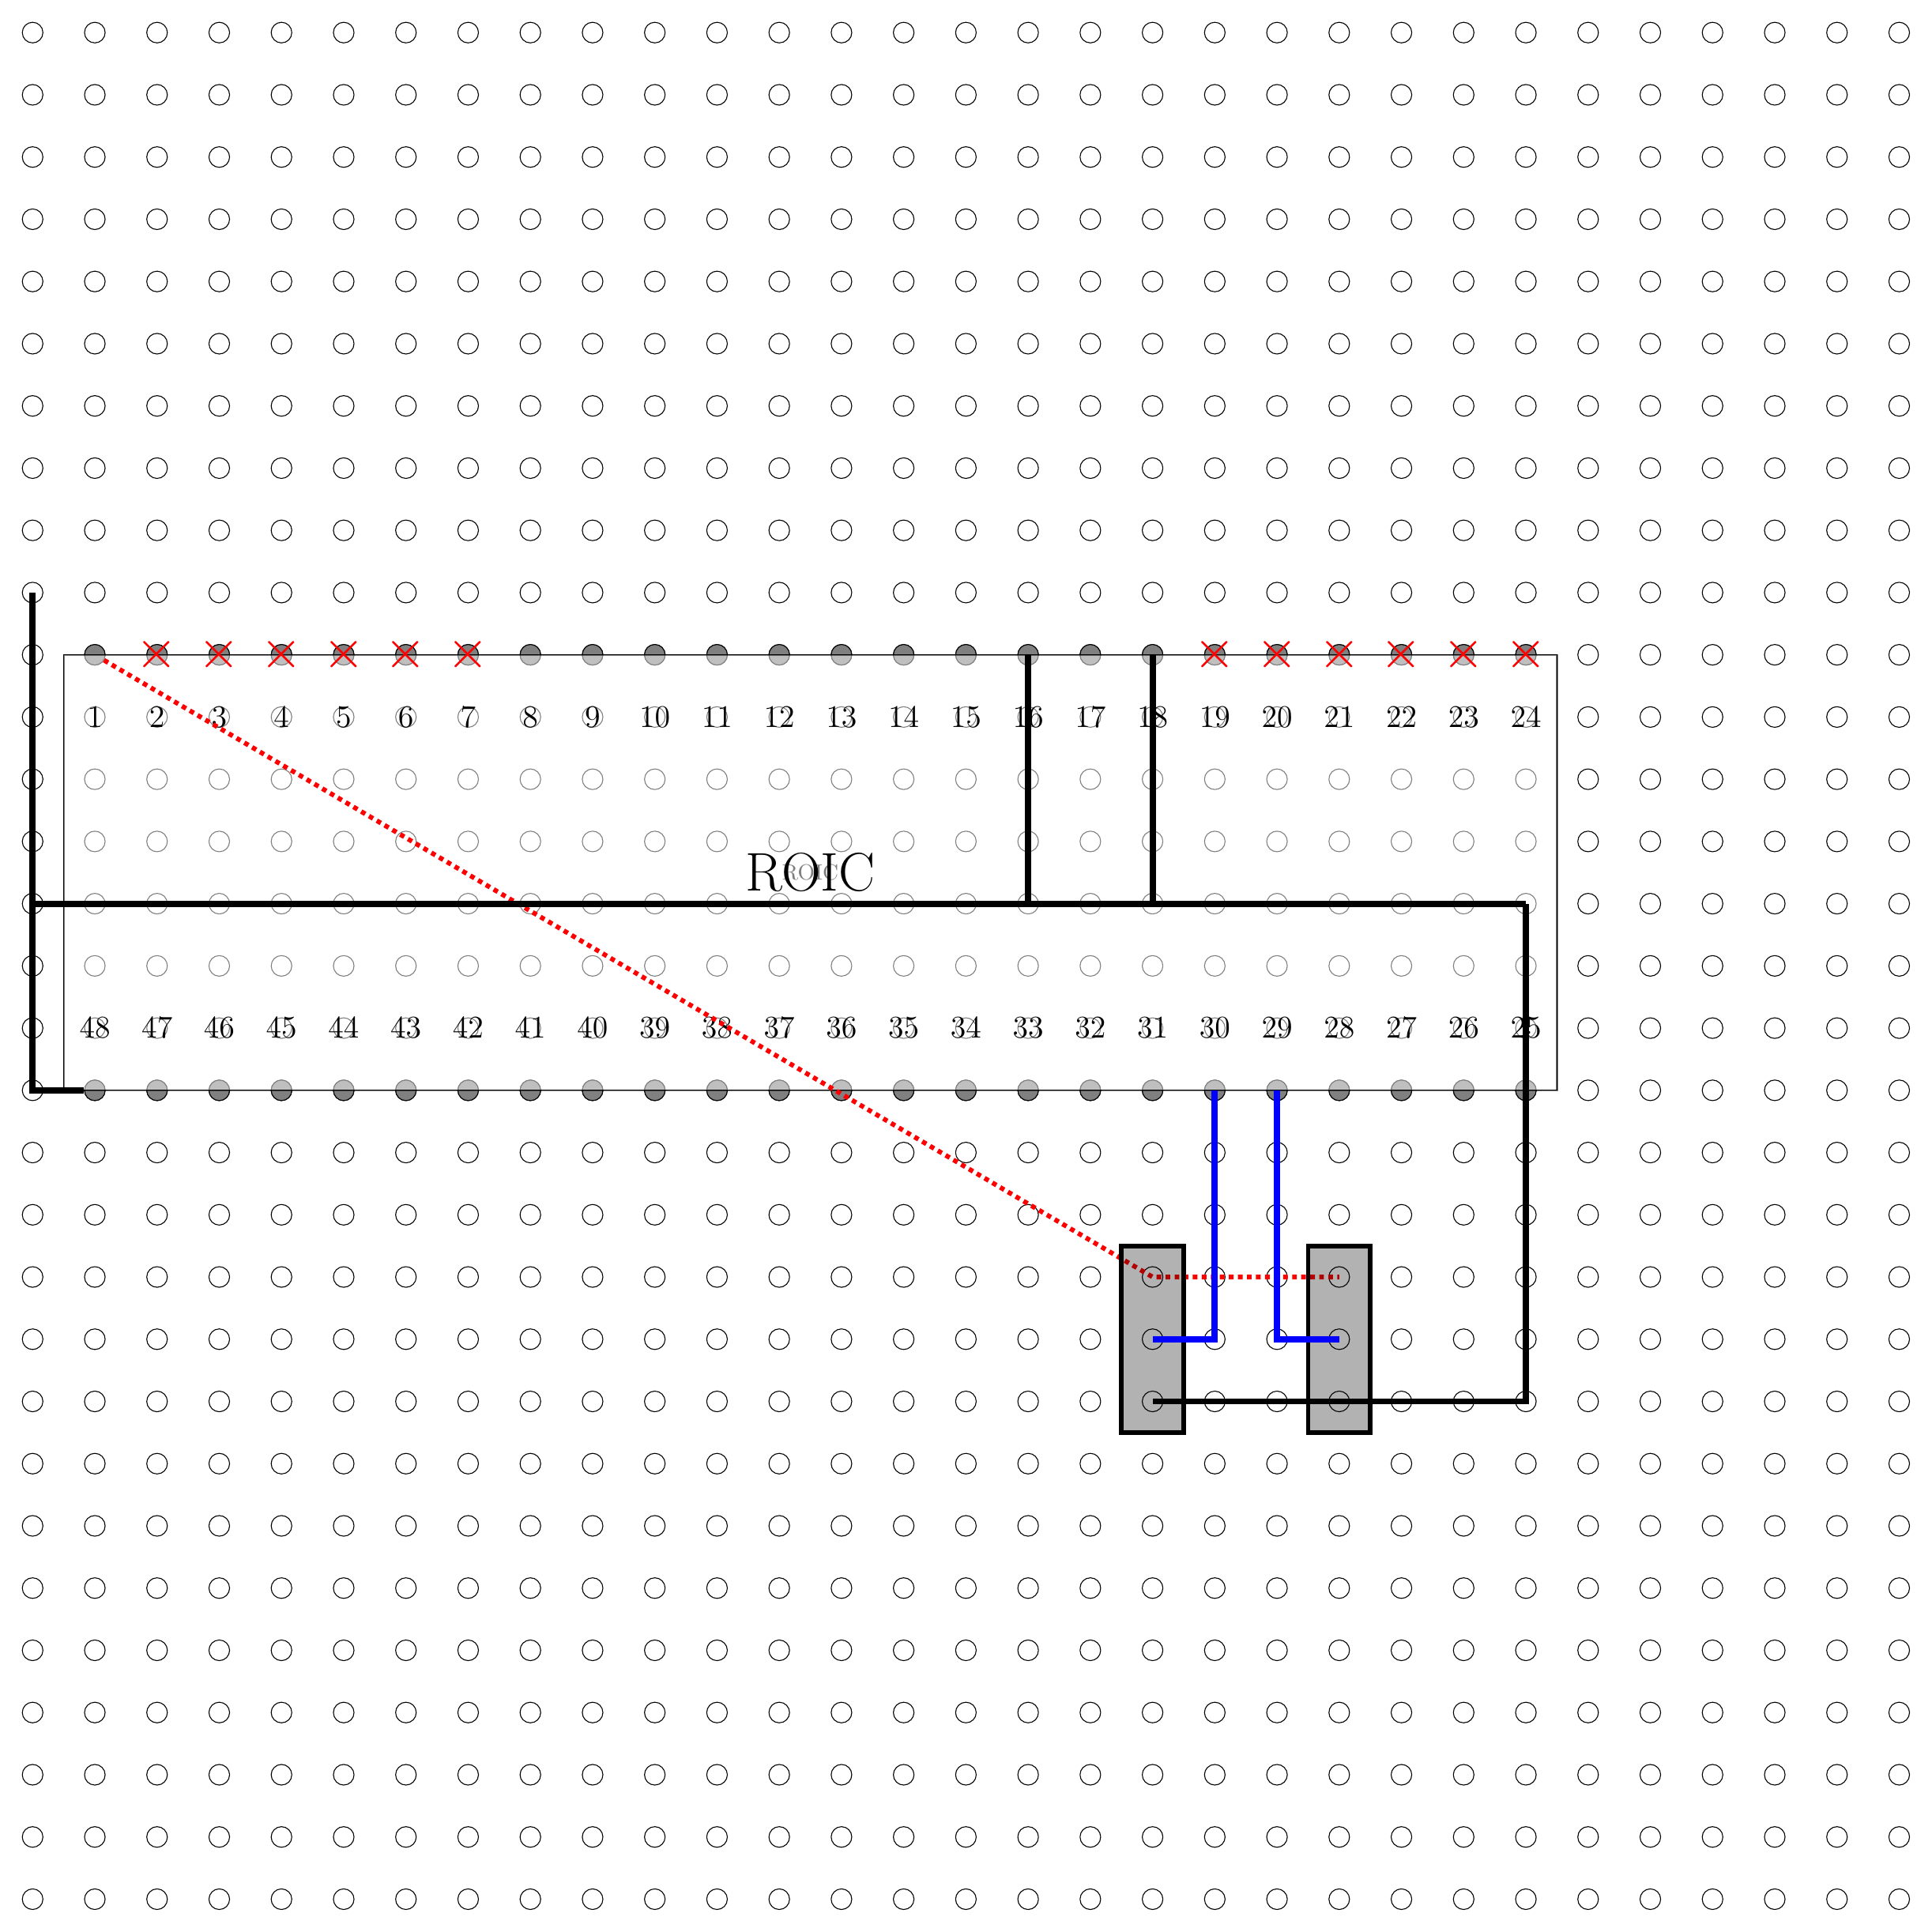
\begin{tikzpicture}[]
%% grid
  \foreach \x in {0,...,30}
    \foreach \y in {0,...,30} 
       {
       \node [gat]  (n\x\y) at (1*\x,1*\y) {};} 
       %\node [gat]  (n\x\y) at (1*\x,1*\y) {\x,\y};}
       
 %% socket
 
\foreach \x in {1,...,24}
 	{\node [pin] (p\x) at (\xstart-1+1*\x,\ystart) {};}

 \foreach \x in {25,...,48}
       {\node [pin] (p\x) at (\xstart+48-\x,\ystart-7) {};}

\draw[fill=white, opacity = 0.5, thick]  (\xstart-.5,\ystart) rectangle (\xstart+23.5,\ystart-7) node[pos=.5]{ROIC};       
\draw[]  (\xstart-0.5,\ystart) rectangle (\xstart+23.5,\ystart-7) node[pos=.5]{\Huge{ROIC}};

 \foreach \x in {1,...,24}
 	{\node [] at (\xstart-1+1*\x,\ystart-1) {\Large{\x}};}

 \foreach \x in {25,...,48}
       {\node [] at (\xstart+48-\x,\ystart-6) {\Large{\x}};}

\node[] at (p2) {\color{red}\Huge{$\times$}};
\node[] at (p3) {\color{red}\Huge{$\times$}};
\node[] at (p4) {\color{red}\Huge{$\times$}};
\node[] at (p5) {\color{red}\Huge{$\times$}};
\node[] at (p6) {\color{red}\Huge{$\times$}};
\node[] at (p7) {\color{red}\Huge{$\times$}};
\node[] at (p19) {\color{red}\Huge{$\times$}};
\node[] at (p20) {\color{red}\Huge{$\times$}};
\node[] at (p21) {\color{red}\Huge{$\times$}};
\node[] at (p22) {\color{red}\Huge{$\times$}};
\node[] at (p23) {\color{red}\Huge{$\times$}};
\node[] at (p24) {\color{red}\Huge{$\times$}};

%% 3.3 V Line
\draw [dotted, line width=.75mm, red ](p1)
to (18,10)
to (21,10);

%% ground
\draw [line width=1mm, black](p48)
to (0,13)
to (0,21)

(0,16) to (24,16)
(16,16) to (16,20)
(18,16) to (18,20)
(24,16) to (24,13)
(24,16) to (24,13)

(24,13) 
to (24,8)
to (18,8)

;


%% capacity switch
\draw [fill, opacity=.3] (20.5,10.5) rectangle (21.5,7.5);
\draw [line width=.75mm] (21.5,7.5) rectangle (20.5,10.5);

\draw [fill, opacity=.3] (17.5,10.5) rectangle (18.5,7.5);
\draw [line width=.75mm] (17.5,10.5) rectangle (18.5,7.5);

\draw [line width=1mm, blue]
(18,9)
to (19,9)
to (19,13)

(21,9)
to (20,9)
to (20,13);

\end{tikzpicture}










\caption{Schematic of breadbord}
\label{tkz:breadbord}
\end{figure}